\documentclass[t]{beamer}
\usetheme[height=7mm]{Rochester}
\setbeamercovered{transparent}
\setbeamertemplate{navigation symbols}{}
%\setbeamertemplate{footline}[frame number]
\setbeamertemplate{footline}
{
\leavevmode%
  \hbox{%
  \begin{beamercolorbox}[wd=\paperwidth,dp=2.5ex,ht=3ex]{}%
    \hspace*{2em}%
    {\hfill Folie \insertframenumber}%
    \hspace*{2em}%
  \end{beamercolorbox}%
  }%
}

\usepackage[german]{babel}
\usepackage[utf8]{inputenc}
\usepackage[linesnumbered,vlined]{algorithm2e}
\DontPrintSemicolon

\theoremstyle{plain}
\newtheorem{Korollar}{Korollar}


\title[Treaps]{Randomisierte Suchstrukturen: Treaps}
\author[M. Beck, R.McDaniel]{Moritz Beck, Robert McDaniel}
\date[10.06.2015]{10. Juni 2015}


\AtBeginSection[]{
    {\setbeamertemplate{footline}{}
    \begin{frame}<beamer>{Gliederung}
        \tableofcontents[currentsection]
    \end{frame}}
}
\AtBeginSubsection[]{
    {\setbeamertemplate{footline}{}
    \begin{frame}<beamer>{Gliederung}
        \tableofcontents[currentsubsection]
    \end{frame}}
}

\beamerdefaultoverlayspecification{<+->}

\begin{document}

{
\setbeamertemplate{footline}{}

\begin{frame}%[plain]
    \titlepage
\end{frame}

\begin{frame}{Gliederung}
    \tableofcontents
\end{frame}
}

\section{Einführung und Motivation}
\subsection{Grundmotivation}
\begin{frame}{Grundmotivation}
    Gesucht: Möglichst schnelle Datenstruktur mit Unterstützung folgender Methoden:
    \bigskip
    \begin{itemize}
        \item<2-> $S$ = MakeSet()
        \item<3-> Insert($i, S$)
        \item<4-> Delete($k, S$)
        \item<5-> Find($k, S$)
        \item<6-> $S$ = Join$(S_1, i, S_2)$
        \item<7-> $S$ = Paste$(S_1, S_2)$
        \item<8-> $S_1, S_2$ = Split$(k, S)$ 
    \end{itemize}
    \bigskip
    \onslide<9-> Bereits bekannt: Binäre Suchbäume
\end{frame}

\subsection{Laufzeiten bei binären Suchbäumen}
\begin{frame}{Laufzeiten bei binären Suchbäumen}
	h = Höhe des Baums
	\begin{table}
	    \begin{tabular}{l | c }
	    Methode & Laufzeit\\
	    \hline
	    $S$ = MakeSet() & $O(1)$\\
	    Insert$(i, S)$ & $O(h)$\\
	    Delete$(k, S)$ & $O(h)$\\
	    Find$(k, S)$ & $O(h)$\\
	    $S$ = Join($S_1, i, S_2$) & STUFF\\
	    $S$ = Paste($S_1, S_2$) & STUFF\\
	    $S_1, S_2$ = Split$(k, S)$ & STUFF
	    %Laufzeiten für Join/Paste/Split?
	    \end{tabular}
	\end{table}
\end{frame}

\subsection{Probleme bei binären Suchbäumen}
	\begin{frame}{Probleme bei binären Suchbäumen}
	\begin{itemize}
	\item Es zeichnet sich ab: Hohe Abhängigkeit von Höhe des Baums $\Rightarrow$ Schwanken zwischen $O(log(n))$ und $O(n)$
	\item Problem: Binärbäume sind oft unoptimal und extreme Fälle führen zu langen Laufzeiten!
	\end{itemize}
	{\only<3->{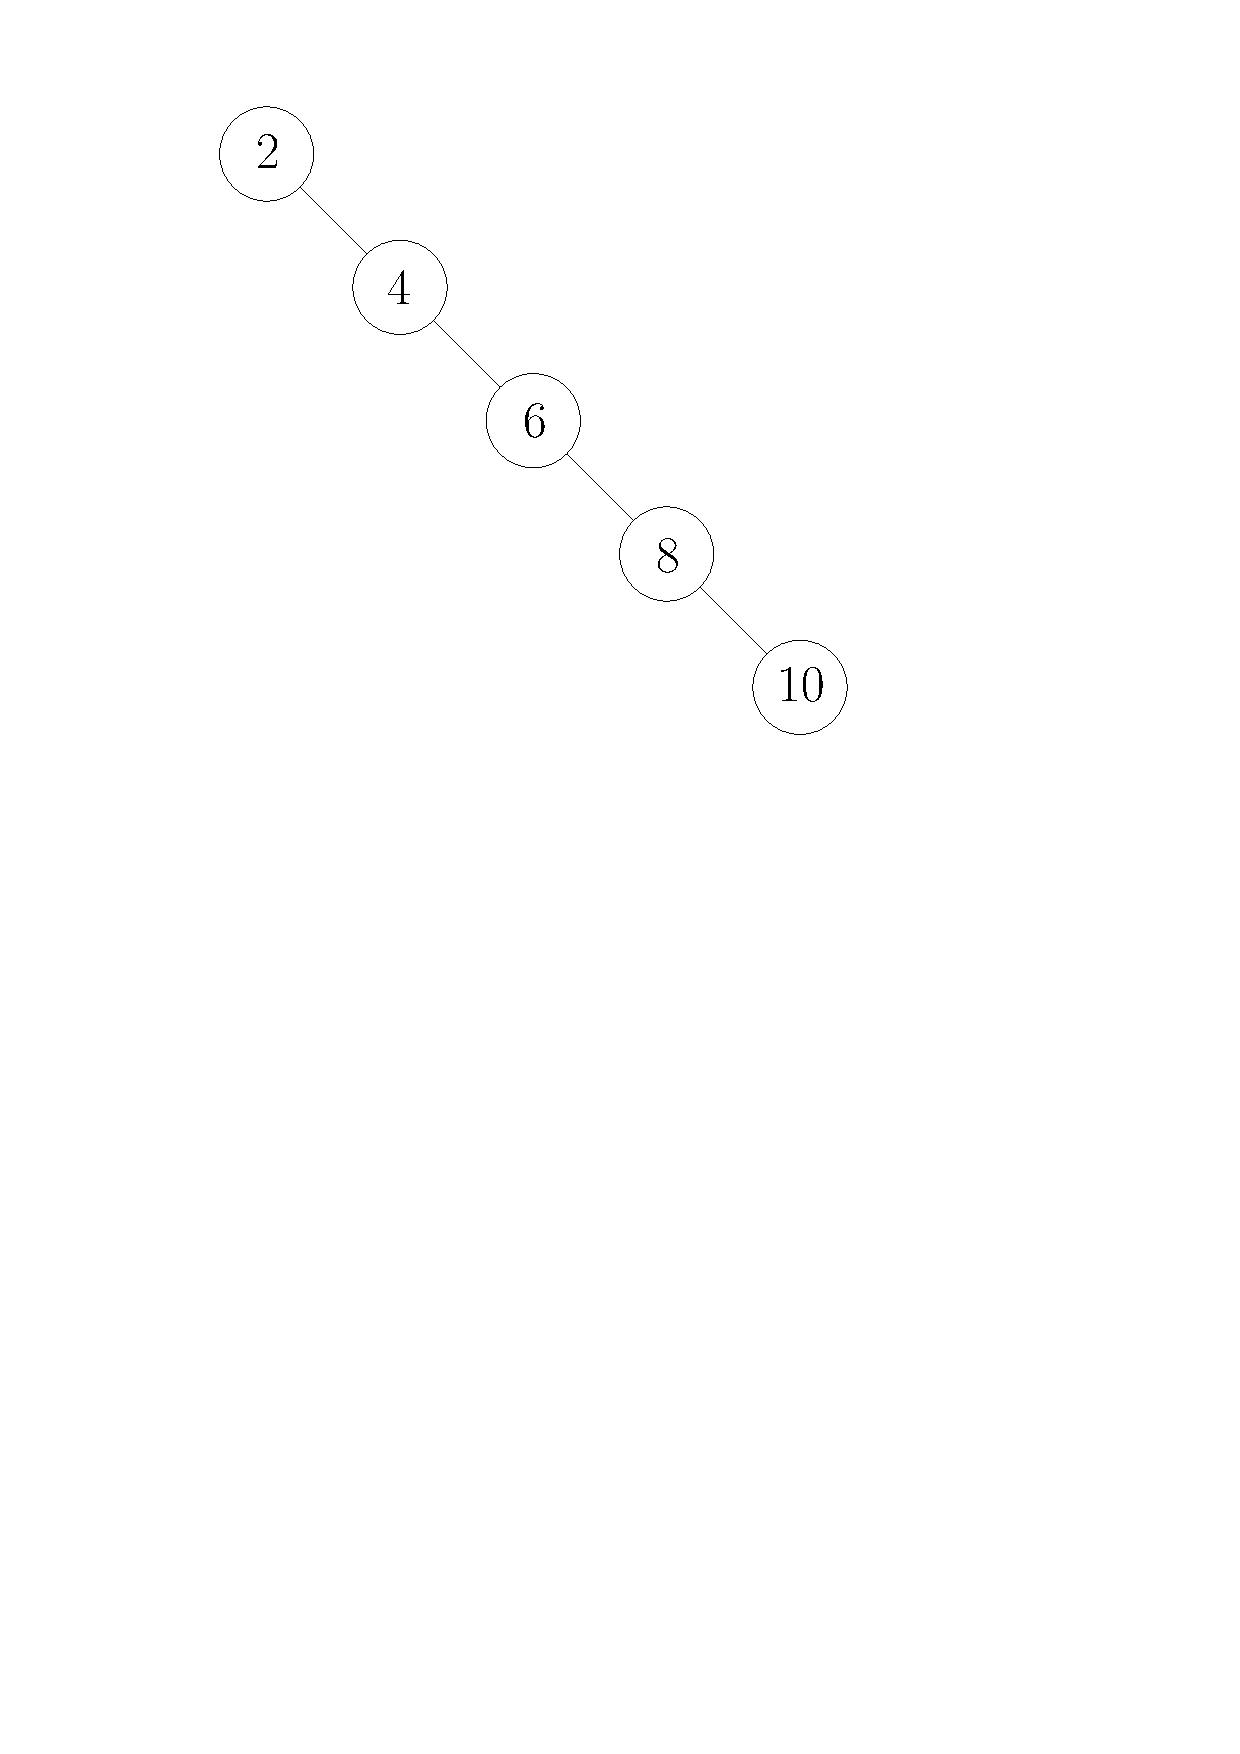
\includegraphics[width=.5\textwidth] {img/BinaryTree.pdf}}}
	%Centering?
\end{frame}

\begin{frame}{Probleme bei binären Suchbäumen}
	\begin{itemize}
	\item Problem: Hohe worst-case-Laufzeiten
	\item Lösung: Vorherige Optimierung (Balancing)?
	\item Implementierung von Balancing bringt neue Probleme:
		\begin{itemize}
		\item Erhöhter Overhead
		\item Höhere Laufzeiten durch konstantes Updating
		\item Speichern von zusätzlicher Information möglicherweise notwendig
		\end{itemize}
	\bigskip
	\item Lösungsidee: Balancing durch Randomisieren?
	\begin{itemize}
		\item Einfache Implementierung
		\item Keine weitere Information zu speichern
		\item Schnelle Ausführung
	\end{itemize}
\end{itemize}
\end{frame}


\section{Treaps}
\subsection{Grundlagen}
\begin{frame}{Titel}
    \begin{center}
        \color{red}{Binary \textbf{Tr}ee} + \color{blue}{H\textbf{eap}} = \textbf{\textcolor{red}{Tr}\textcolor{blue}{eap}}
    \end{center}
    \begin{itemize}
        \item<2-> \textcolor{red}{Schlüssel}
        \item<3-> \textcolor{blue}{Priorität} (meist Implementierungsdetail)
    \end{itemize}
    \vspace{1em}
    \hfill\only<4->{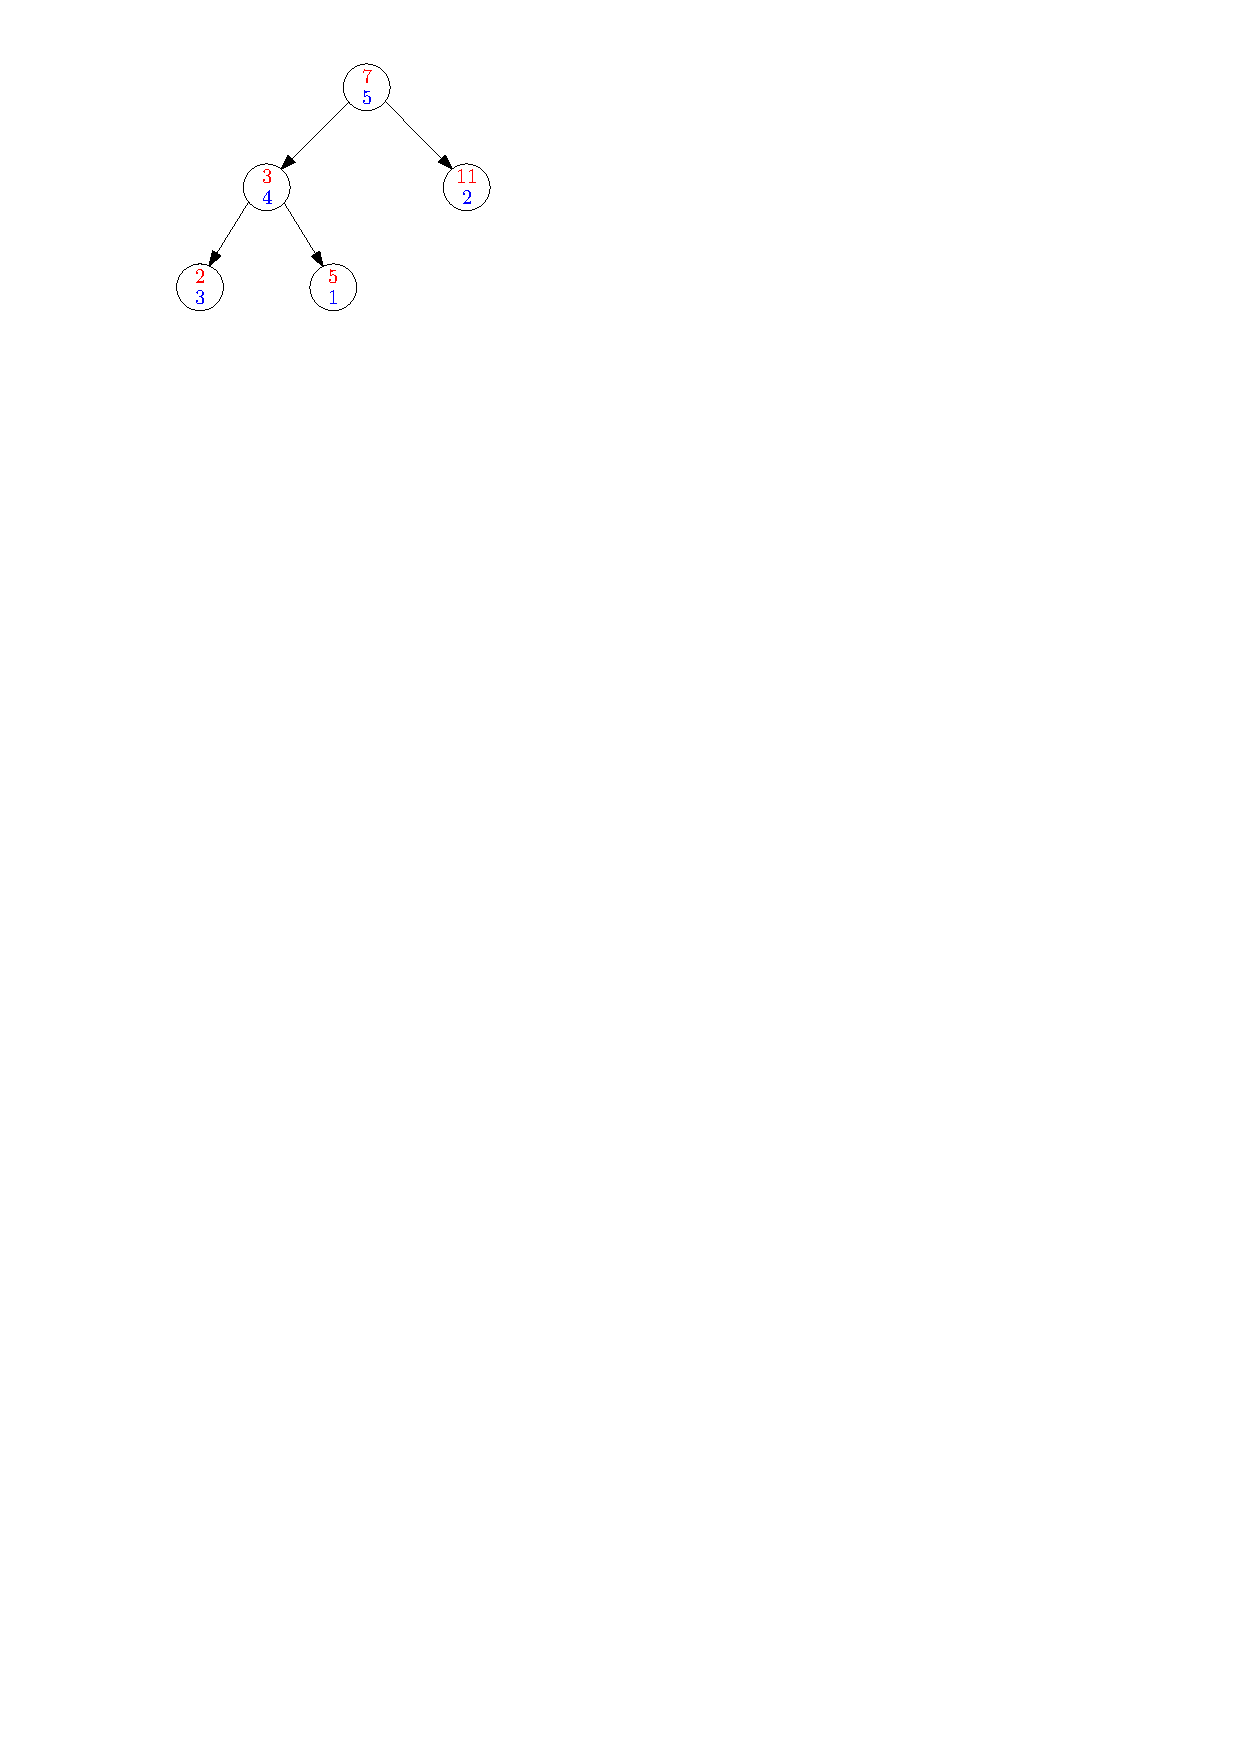
\includegraphics[page=1,width=.5\textwidth]{img/Beispiel_Treap.pdf}}
\end{frame}

\subsection{Existenz eindeutiger Treaps}
\begin{frame}{Titel}
    \begin{Satz}
        Für jede Menge $M$ von Schlüssel-Priorität-Paaren mit paarweise unterschiedlichen Schlüsseln und Prioritäten existiert genau ein gültiger Treap.
    \end{Satz}
    \begin{proof}
        Per Induktion über $\left|M\right|$:
        \raisebox{3em}{\begin{columns}<2->
            \begin{column}[t]{.65\textwidth}
                \begin{itemize}
                \item<3-> \textbf{IA}: leere Menge $\leftrightarrow$ leerer Baum \textcolor[rgb]{0,.7,0}{\Large\checkmark}
                \item<4-> \textbf{IS}: $t   = \{(k, p) \in M \mid p \text{ minimal}\}$
                                       $M_< = \{(k, p) \in M \mid k < t_k\}$ \\
                                       $M_> = \{(k, p) \in M \mid k > t_k\}$
                \end{itemize}
            \end{column}
            \begin{column}[t]{0.35\textwidth}
                \raisebox{-\totalheight}{\visible<5->{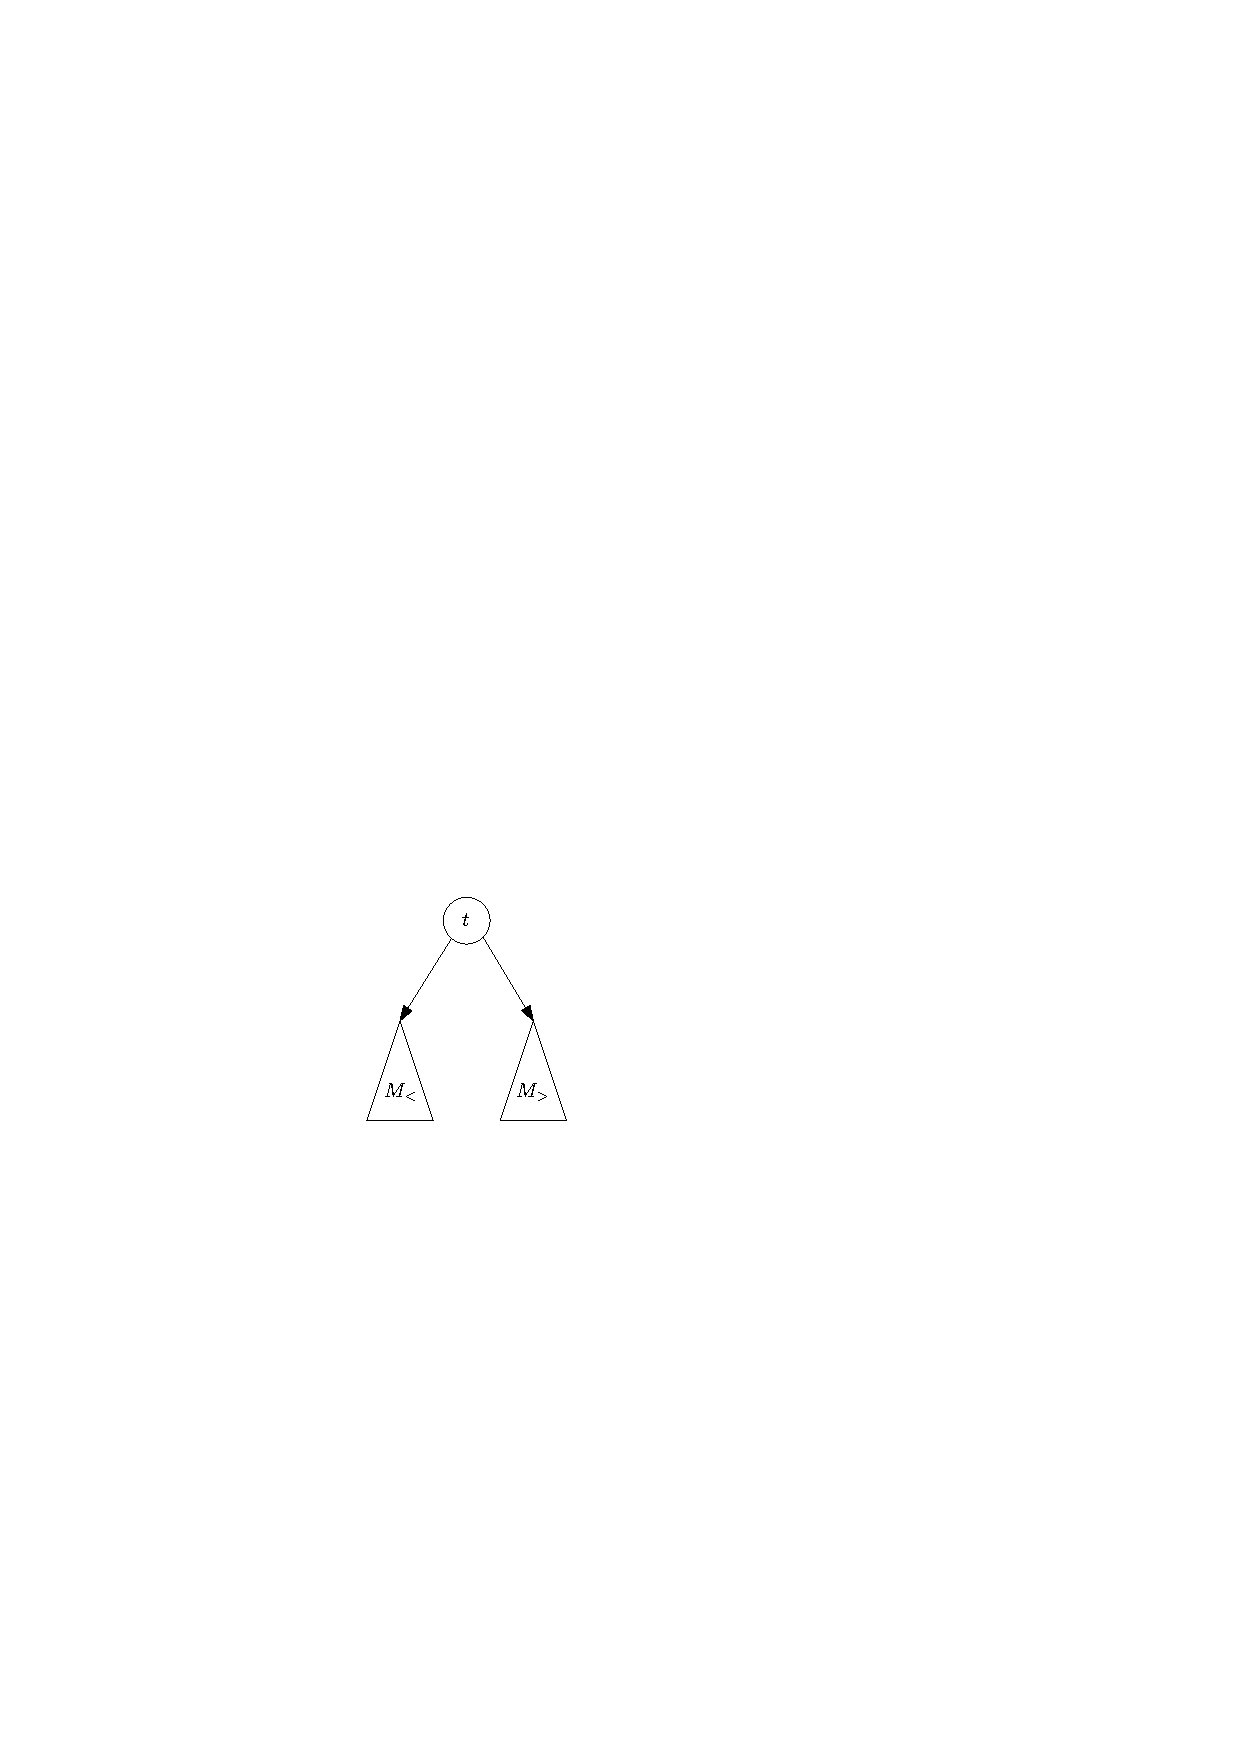
\includegraphics[width=.9\textwidth]{img/Eindeutigkeit_IS.pdf}}}
                %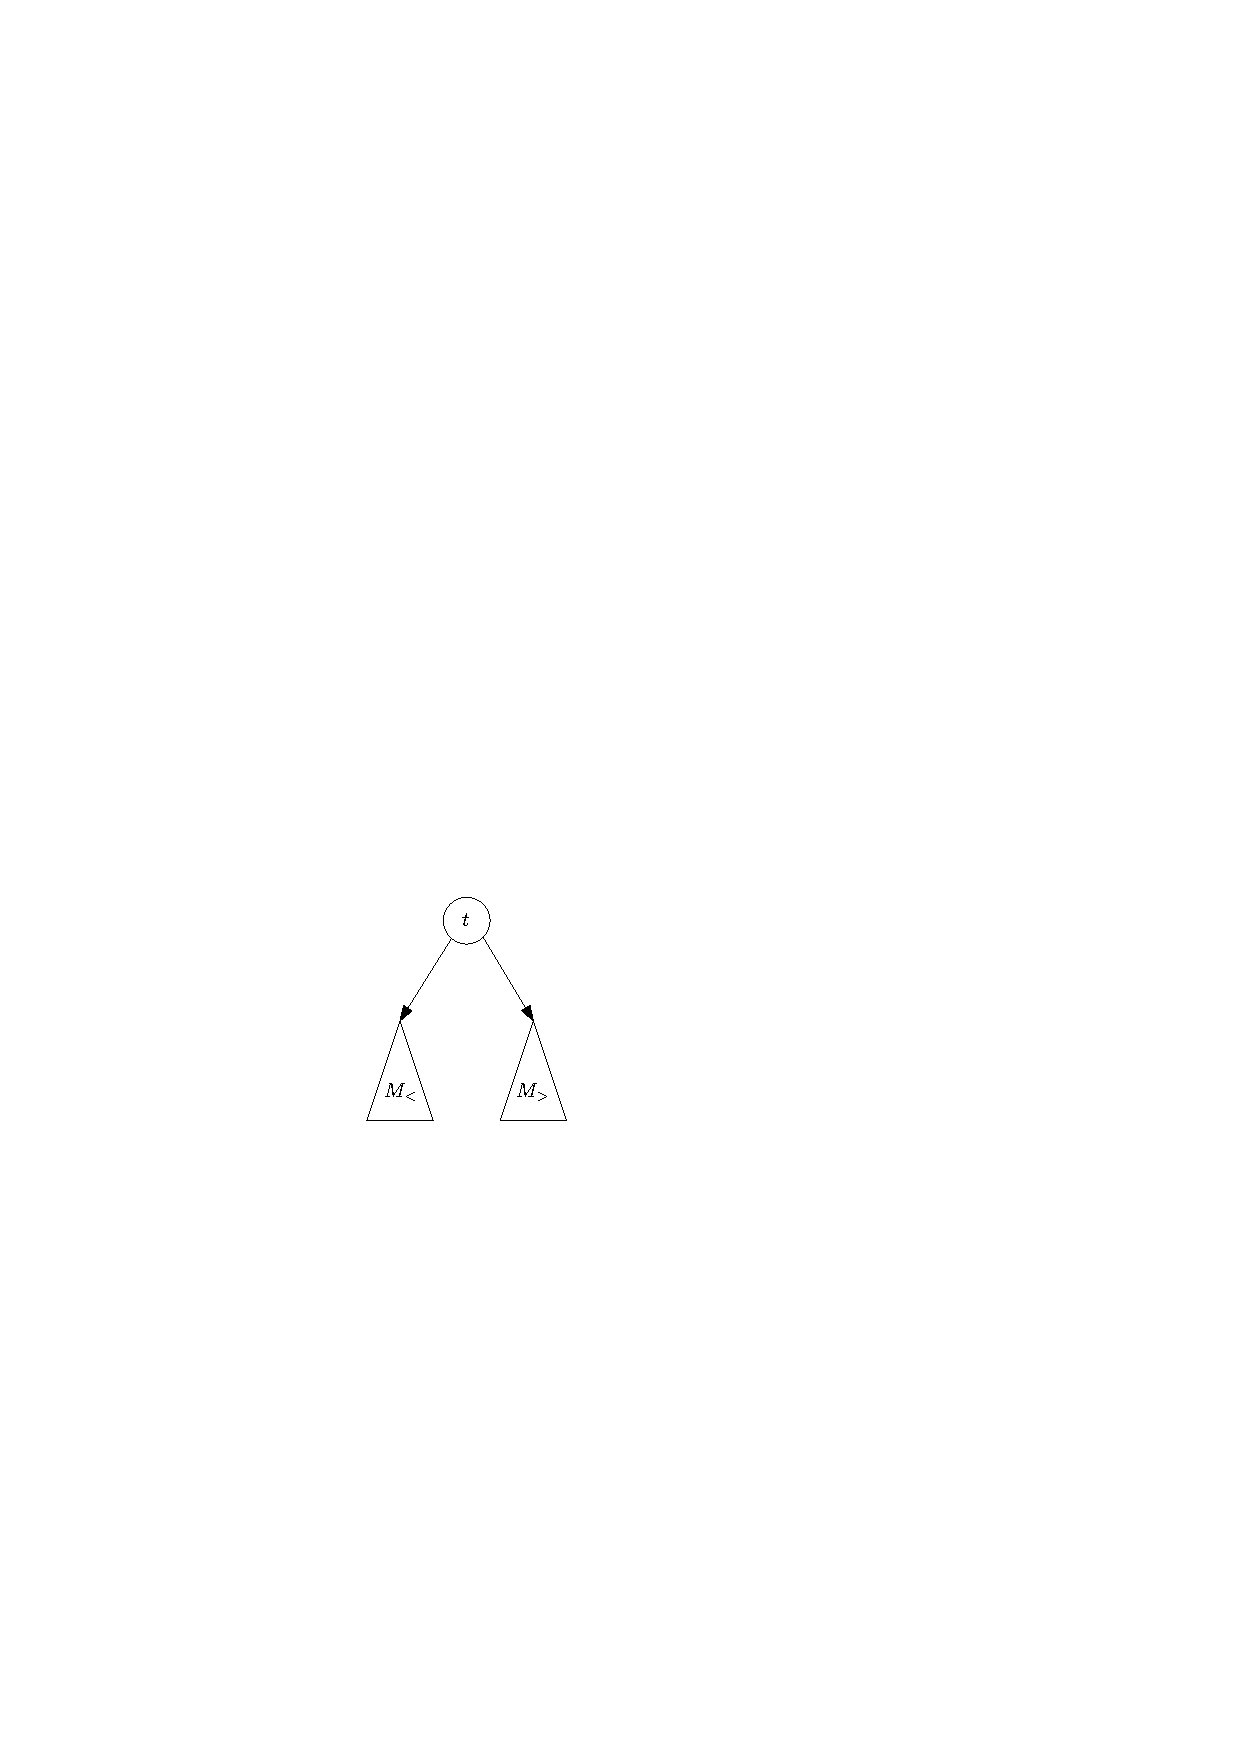
\includegraphics[width=.9\textwidth]{img/Eindeutigkeit_IS.pdf}
            \end{column}
        \end{columns}}
    \end{proof}
\end{frame}

\subsection{Implementierung}
\begin{frame}{Titel}
    
\end{frame}

\subsection{Laufzeitanalyse}
\begin{frame}{Titel}
    
\end{frame}


\section*{Fazit}
\begin{frame}{Fazit}
    
\end{frame}



% \section{Skip-Lists}
% \subsection{Grundlagen}
% \begin{frame}{Titel}
    
% \end{frame}

% \section*{Ende}
% {\setbeamertemplate{footline}{}
% \begin{frame}<beamer>[c]
    % \begin{center}
    % \Huge{Fragen?}
    % \end{center}
% \end{frame}}

\end{document}